\documentclass{article}

% Encodings, page setup, paragraph formatting, font
\usepackage[top=0.9in, bottom=1in, left=1.5in, right=1.5in]{geometry}
\usepackage[icelandic]{babel}
\usepackage[T1]{fontenc}
\usepackage[sc]{mathpazo}
\usepackage[parfill]{parskip}
\usepackage{cancel}
% Tables and lists
\usepackage{booktabs,tabularx}
\usepackage{multirow}
\usepackage{enumerate}
\usepackage{adjustbox}
\usepackage{multicol}
\usepackage{enumitem}
\usepackage{xcolor}
% Math
\usepackage{amsmath, amsfonts, amssymb, amsthm}
% Graphics
\usepackage{graphicx}
\usepackage{forest}
\usepackage{tikz}
\usetikzlibrary{positioning, shapes, arrows.meta}


\usepackage{listingsutf8}
\definecolor{commentcolor}{RGB}{255, 0, 255} % Bleikur
\definecolor{keywordcolor}{RGB}{139, 69, 19}   % Brúnn
\definecolor{stringcolor}{RGB}{0, 0, 255}      % Blár
\definecolor{numbercolor}{RGB}{0, 128, 0}      % Grænn
\definecolor{identifiercolor}{RGB}{0, 0, 255}
%Morpho
\lstdefinelanguage{CustomLang}{
    alsoletter={=},
    keywords={rec, fun, if, else, return},
    sensitive=true,
    comment=[l]{;;;},
    commentstyle=\color{commentcolor},
    morestring=[b]",
    stringstyle=\color{stringcolor},
}

\lstset{
    language=CustomLang,
    basicstyle=\ttfamily,
    keywordstyle=\color{keywordcolor},
    commentstyle=\color{commentcolor},
    identifierstyle=\color{identifiercolor},
    stringstyle=\color{stringcolor},   
    showstringspaces=false,
    numbers=none,
    tabsize=2,
    breaklines=true,
    columns=fullflexible,
    keepspaces=true,
    inputencoding=utf8, 
    extendedchars=true,  
    literate=
        {á}{{\'a}}1
        {ð}{{\dh}}1
        {é}{{\'e}}1
        {í}{{\'i}}1
        {ó}{{\'o}}1
        {ú}{{\'u}}1
        {ý}{{\'y}}1
        {þ}{{\th}}1
        {æ}{{\ae}}1
        {ö}{{\"o}}1
        {Á}{{\'A}}1
        {Ð}{{\DH}}1
        {É}{{\'E}}1
        {Í}{{\'I}}1
        {Ó}{{\'O}}1
        {Ú}{{\'U}}1
        {Ý}{{\'Y}}1
        {Þ}{{\TH}}1
        {Æ}{{\AE}}1
        {Ö}{{\"O}}1,
}


% Hyphenation
\hyphenpenalty=5000
% Page and section numbering
\setcounter{secnumdepth}{-1} 
\pagenumbering{gobble}
\title{Forritunarmál}
\author{Benjamín}
\date{11.27.2024}

\begin{document}

\maketitle
\begin{center}

\Huge{\textbf{TÖL304G Final Exam}}


\LARGE{\textbf{TÖL304 Lokapróf}}

\vspace{5em}


\includegraphics[scale = 0.5]{myndir/bugun.jpg}
\end{center}


\newpage


\begin{center}
    \textbf{Hluti I - Bálkmótun o.fl.}

    \textbf{Svarið að minnsta kosti tveimur spurningum í þessum hluti - Munið að svara a.m.k. 10 spurningum í heild}
\end{center}

\section{1.}

Hverjar eftirfarandi fullytðinga um lokanir eru sannar? Tvö röng svör gefa núll punkta.

\begin{itemize}
    \item[a)] Lokanir innihalda fallsbendi.
    \item[b)] Lokanir eru til í C.
    \item[c)] Lokanir eru til í Scheme.
    \item[d)] Lokanir eru til í CAML.
    \item[e)] Lokanir eru til í Morpho.
    \item[f)] Lokanir eru aðeins mögulegar ef vakningarfærslur eru í kös.
    \item[g)] Lokanir má nota til að utfæra strauma í Scheme.
    \item[h)] Lokanir innihalda tengihlekk(aðgangshlekk).
    \item[i)] Lokanir innihalda stýrihlekk.
    \item[j)] Lokanir innihalda straum.  
    \item[k)] Lokanir eru nauðsynlegar til að skila staðværu falli sem skilagildi falls í bálkmótuðum forritunarmálum.
    \item[l)] Lokanir eru nauðsynlegat til að senda staðvær föll sem viðföng í föll í bálkmótuðum forritunarmálum.        
\end{itemize}

\textbf{Svar}:

\begin{tabularx}{\textwidth}{ |X|X|X|X|X|X|X|X|X|X|X|X|}
   \hline
   \textbf{a} & \textbf{b} & \textbf{c}  & \textbf{d} & \textbf{e}  & \textbf{f}  & \textbf{g}  & \textbf{h}  & \textbf{i}  & \textbf{j}  & \textbf{k}  & \textbf{l}  \\ \hline
    & & & & & & & & & & & \\ \hline
    
\end{tabularx}


\newpage

\section{2.}

Vakningarfærsla falls í bálkmótuðu forritunarmáli eins og Scheme inniheldur sum eftirfarandi atriða.
Hver? Eitt rangt svar gefur \underline{núll} stig.

\begin{enumerate}[label = \alph*)]
    \item Staðværar breytur fallsins.
    \item Staðværar breytur fallsins sem kallaði á fallið.
    \item Víðværar breytur sem eru aðgengilegar í fallinu.
    \item Skráarkerfi tölvunnar.
    \item Viðföng fallsins.
    \item Aðgangshlekk (tengihlekk).
    \item Stýrihlekk.
    \item Vendivistfang.
    \item Benda á öll föll sem hægt er að kalla á úr fallinu.
    \item Benda á allar lifandi vakningarfærslur.
    \item Alla hluti sem eru í kerfinu.
    \item Vakningarfærslur allra falla sem hægt er að kalla á.
    \item Nöfn allra falla sem hægt er að kalla á.
\end{enumerate}

\textbf{Svar}:

\begin{tabularx}{\textwidth}{ |X|X|X|X|X|X|X|X|X|X|X|X|X|}
    \hline
    \textbf{a}  & \textbf{b}  & \textbf{c}  & \textbf{d}  & \textbf{e}  & \textbf{f}  & \textbf{g}  & \textbf{h}  & \textbf{i}  & \textbf{j}  & \textbf{k}  & \textbf{l} & \textbf{m}   \\ \hline
     & & & & & & & & & & & & \\ \hline
 \end{tabularx}

 \newpage

 \section{3.}
    Vakningarfærsla falls í bálkmótuðu forritunarmáli eins og Scheme inniheldur sum eftirfarandi atriða. Hver? Eitt rangt svar gefur \underline{núll} sitg.

    \begin{enumerate}[label = \alph*)]
        \item Staðværar breytur fallsins.
        \item Staðværar breytur fallsins sem kallaði á fallið
        \item Víðvlrar breytur sem eru aðgengilegar i fallinu.
        \item Skraarkerfi tölvunnar.
        \item viðföng fallsins.
        \item Aðgangshlekk (tengihlekk).
        \item Stýrihlekk.
        \item Vendivistfang.
        \item Benda á öll föll sem hægt er að kalla á úr fallinu.
        \item Benda á allar lifandi vakningarfærslur. 
        \item Alla hlutina sem til eru í kerfinu.
        \item Vakningarfærslur allra falla sem hægt er að kalla á.
        \item Nöfn allra falla sem hægt er að kalla á.
    \end{enumerate}

    \textbf{Svar}:

    \begin{tabularx}{\textwidth}{ |X|X|X|X|X|X|X|X|X|X|X|X|X|}
        \hline
        \textbf{a}  & \textbf{b}  & \textbf{c}  & \textbf{d}  & \textbf{e}  & \textbf{f}  & \textbf{g}  & \textbf{h}  & \textbf{i}  & \textbf{j}  & \textbf{k}  & \textbf{l} & \textbf{m}   \\ \hline
         & & & & & & & & & & & & \\ \hline
     \end{tabularx}

     \newpage

     \section{4.}
     Íhugið myndina sem sýnir földun falla P, Q, R, S og T.

     \begin{center}
        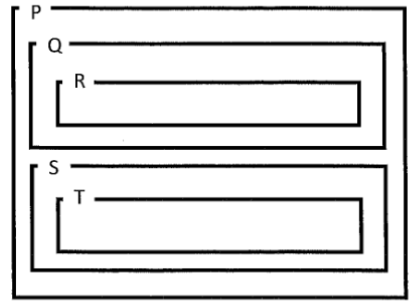
\includegraphics[scale = 1]{myndir/foldun.png}
     \end{center}

     Samsvarandi Scheme forritstexti er einnig sýndur í tveimur jafngildum útgáfum 
     hlið við hlið. 

     \begin{verbatim}
    (define ( P...)                        (define(P ...)
     (define (Q ...)                        (define(S ...)
      (define (R ...)                        (define (T...)
       ...[stifn R/body of R]                  ...[stofn T/body of T]
      )                                      )
      ...[stofn Q/body of Q]                 ...[stofn S/body of S]
     )                                      )
     (define (S ...)                        (define (Q ...)
      (define (T...)                         (define (R ...)
       ...[stofn T/body of T]                 ...[stofn R/body of R]
      )                                      )
      ...[stofn S/body of S]                 ...[stofn Q/body of Q]
     )                                      )
     ...[stofn P/body of P]                 ...[stofn P/body of P]
    )                                       )
     \end{verbatim}
    
     Fyllið út eftirfarandi töflur með því að setja krossa við sannar fullyrðingar.
     Eitt rangt svar gefur \underline{núll} í einkunn fyrir dæmið.

     \textbf{Svar}:

     kalla má á P úr:


     \begin{tabularx}{\textwidth}{ |X|X|X|X|X|}
        \hline
        \textbf{P}  & \textbf{Q}  & \textbf{R}  & \textbf{S}  & \textbf{T} \\ \hline
         & & & & \\ \hline
     \end{tabularx}


     kalla má á Q úr:

     
     \begin{tabularx}{\textwidth}{ |X|X|X|X|X|}
        \hline
        \textbf{P}  & \textbf{Q}  & \textbf{R}  & \textbf{S}  & \textbf{T} \\ \hline
         & & & & \\ \hline
     \end{tabularx}


     kalla má á R úr:

     
     \begin{tabularx}{\textwidth}{ |X|X|X|X|X|}
        \hline
        \textbf{P}  & \textbf{Q}  & \textbf{R}  & \textbf{S}  & \textbf{T} \\ \hline
         & & & & \\ \hline
     \end{tabularx}

     kalla má á S úr:

     
     \begin{tabularx}{\textwidth}{ |X|X|X|X|X|}
        \hline
        \textbf{P}  & \textbf{Q}  & \textbf{R}  & \textbf{S}  & \textbf{T} \\ \hline
         & & & & \\ \hline
     \end{tabularx}

     kalla má á T úr:

     
     \begin{tabularx}{\textwidth}{ |X|X|X|X|X|}
        \hline
        \textbf{P}  & \textbf{Q}  & \textbf{R}  & \textbf{S}  & \textbf{T} \\ \hline
         & & & & \\ \hline
     \end{tabularx}

     Staðværar breytur í P má nota í:

     
     \begin{tabularx}{\textwidth}{ |X|X|X|X|X|}
        \hline
        \textbf{P}  & \textbf{Q}  & \textbf{R}  & \textbf{S}  & \textbf{T} \\ \hline
         & & & & \\ \hline
     \end{tabularx}


     Staðværar breytur í Q má nota í:

     
     \begin{tabularx}{\textwidth}{ |X|X|X|X|X|}
        \hline
        \textbf{P}  & \textbf{Q}  & \textbf{R}  & \textbf{S}  & \textbf{T} \\ \hline
         & & & & \\ \hline
     \end{tabularx}


     Staðværar breytur í R má nota í:

     
     \begin{tabularx}{\textwidth}{ |X|X|X|X|X|}
        \hline
        \textbf{P}  & \textbf{Q}  & \textbf{R}  & \textbf{S}  & \textbf{T} \\ \hline
         & & & & \\ \hline
     \end{tabularx}



     Staðværar breytur í S má nota í:

     
     \begin{tabularx}{\textwidth}{ |X|X|X|X|X|}
        \hline
        \textbf{P}  & \textbf{Q}  & \textbf{R}  & \textbf{S}  & \textbf{T} \\ \hline
         & & & & \\ \hline
     \end{tabularx}


     \newpage

     \section{5.}
     Eftirfarandi forritstexti er í einhverju ímynduðu forritunarmáli.
     \begin{verbatim}
        void f(x,y)
        {
            y = 3;
            print x,y;
            x = 2;
        }
        int i,a[10];
        for(int i= 0; i != 10; i++) a[i] = i +1;
        f(a[a[0]],a[0]);
        print a[0], a[1], a[2], a[3];
     \end{verbatim}

     Hvað skrifar þetta forrit (sex gildi í hvert skipti) ef viðföngin eru:

     \subsection{a)} Gildisviðföng 

     \subsection{b)} Tilvísunarviðföng

     \subsection{c)} Nafnviðföng


     \newpage

     \begin{center}
        \textbf{Hluti II - Listavinnsla o.fl.}


        \textbf{Svarið að minnsta kosti tveimur spurningum i þessum hluta - Munið að svara a.m.k. 10 spurningum í heild}
     \end{center}

     \section{6.}
     Skrifið fall í Scheme, Caml, Morpho eða Haskell sem tekur eitt viðfang sem er listi lista af fleytitölum milli 0 og 1 og skilar tölu sem 
     er stærsta lággildi innri listanna, þ.e. stærst af þeim tölum sem fást 
     þegar fundinn er minnsta tala í hverjum innri lista. Þið skuluð reikna
     með því að hágildi í tóma menginu sé 0 og lággildi í tóma menginu sé 1.
     Munið fallslýsingar, eing og alltaf. Fallið þarf að skila viðeigandi 
     gildi bæði fyrir toman lista og fyrir lista sem einungis inniheldur tóma lista.

     \textbf{Svar:}



     \newpage 

     \section{7.}

     Skrifið fall Zip2 i Sheme, CAML, Morpho eða Haskell sem tekur 
     tvíundaraðgerð (fall) og tvo jafnlanga lista sem viðföng og skilar lista þeirra útkomna sem fást þegar tvíundaraðgerðinni er beitt á
     gildin


\begin{lstlisting}
;;; Notkun:
;;; Fyrir:
;;;
;;; Gildi:
writeln("Hello world");  
\end{lstlisting}

\end{document}